\chapter{Membuat Aplikasi di Oracle Application Express (APEX)}

Pertama yang harus dilakukan adalah membuat workspace di oracle. Kemudian sign ke workspace yang telah dibuat. kemudian pilih app builder, lalu pilih create. Dimenu berikutnya pilih untuk memasukan file data tabel mahasiswa xls. beri nama tabel, lalu klik load data, setelah load data klik create aplication. aplikasi sudah dibuat untuk mengeceknya bisa dilakukan dengan menrunning aplikasi tersebut. Berikut urutan langkah-langkah dalam bentuk gambarnya.\\

\begin{figure}[H]
	\centering
	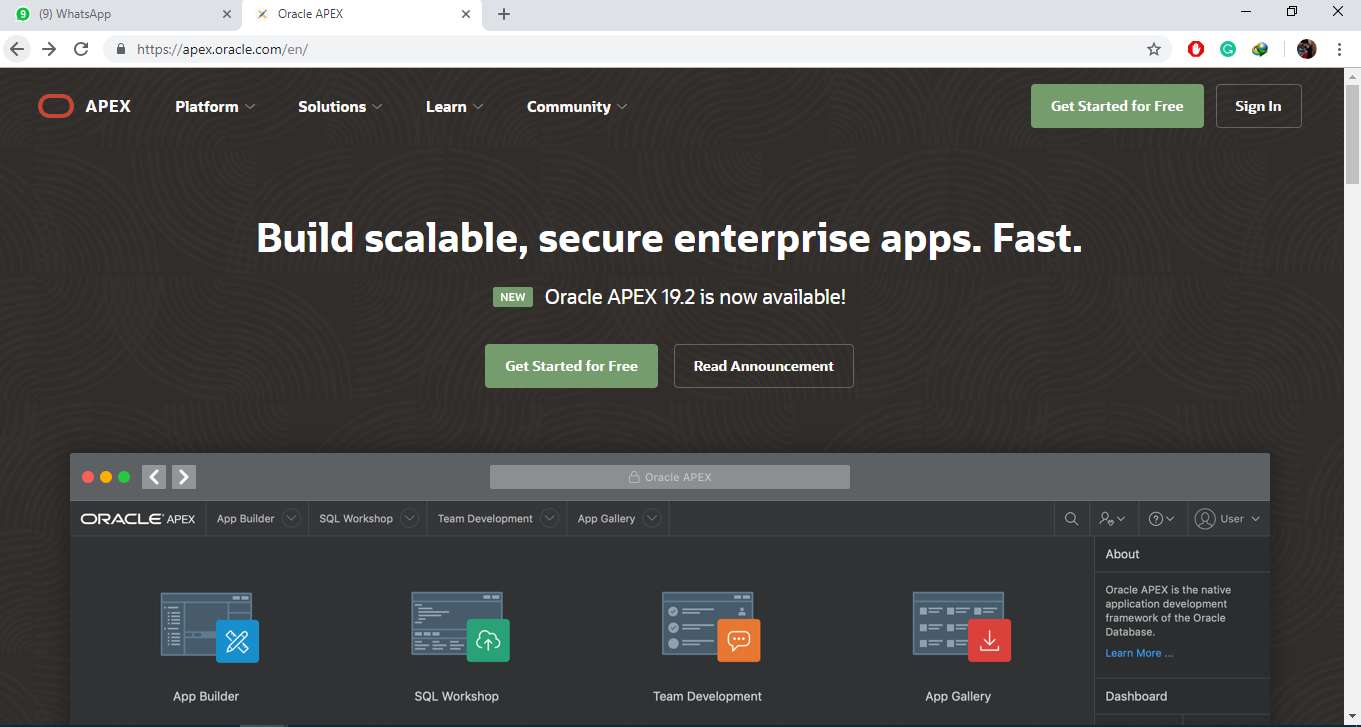
\includegraphics[width=8cm]{figures/1.png}
\end{figure}

\begin{figure}[H]
	\centering
	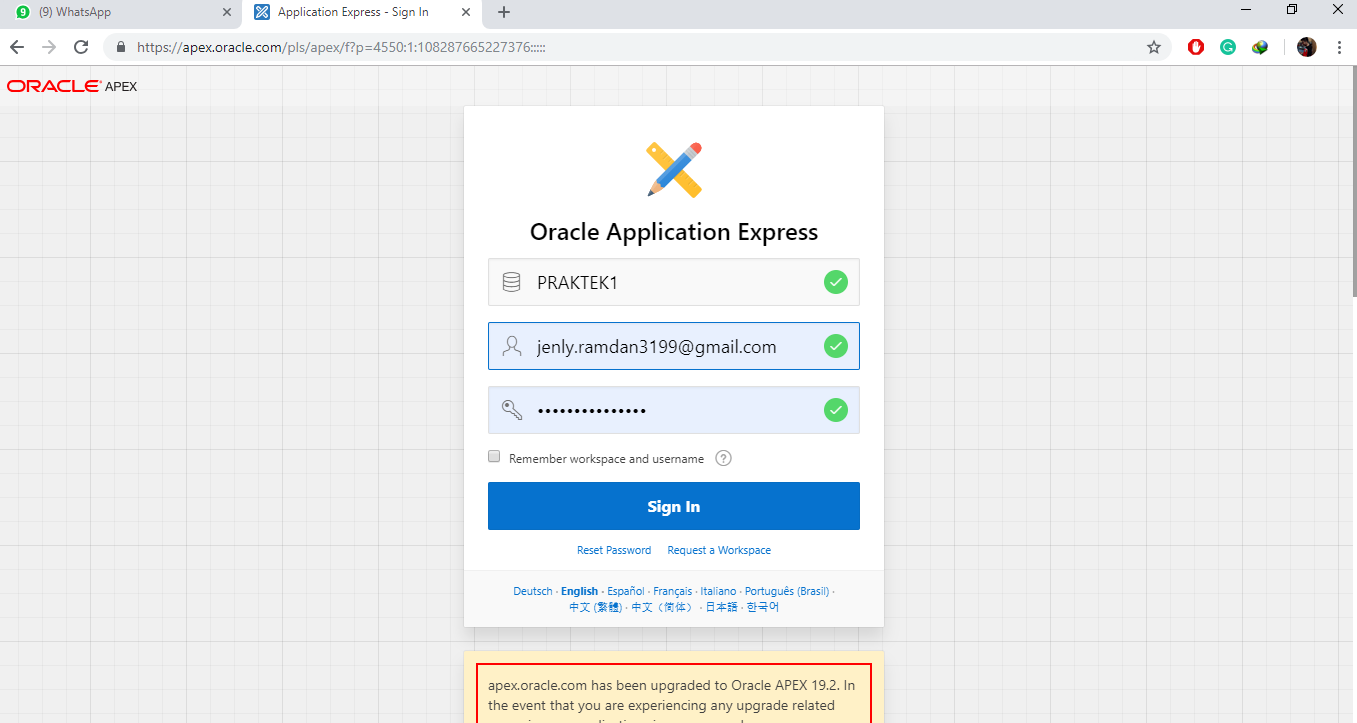
\includegraphics[width=8cm]{figures/2.png}
\end{figure}

\begin{figure}[H]
	\centering
	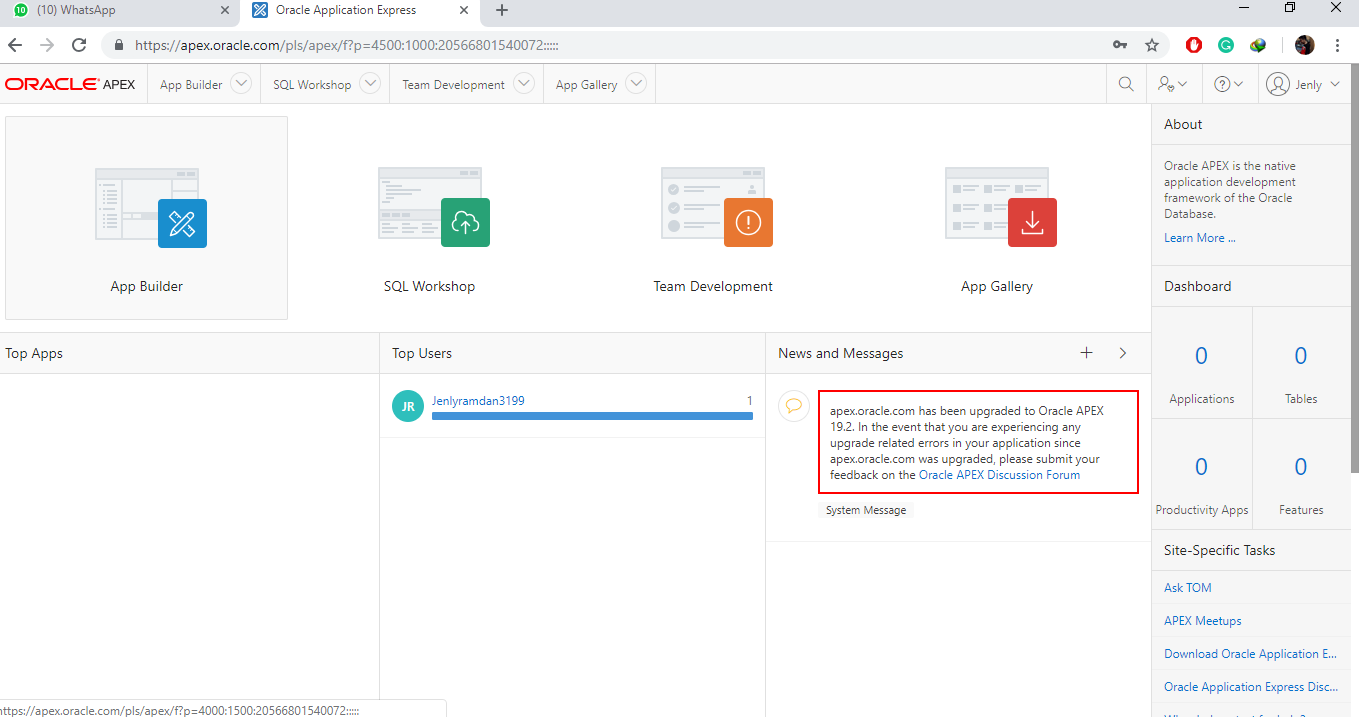
\includegraphics[width=8cm]{figures/3.png}
\end{figure}

\begin{figure}[H]
	\centering
	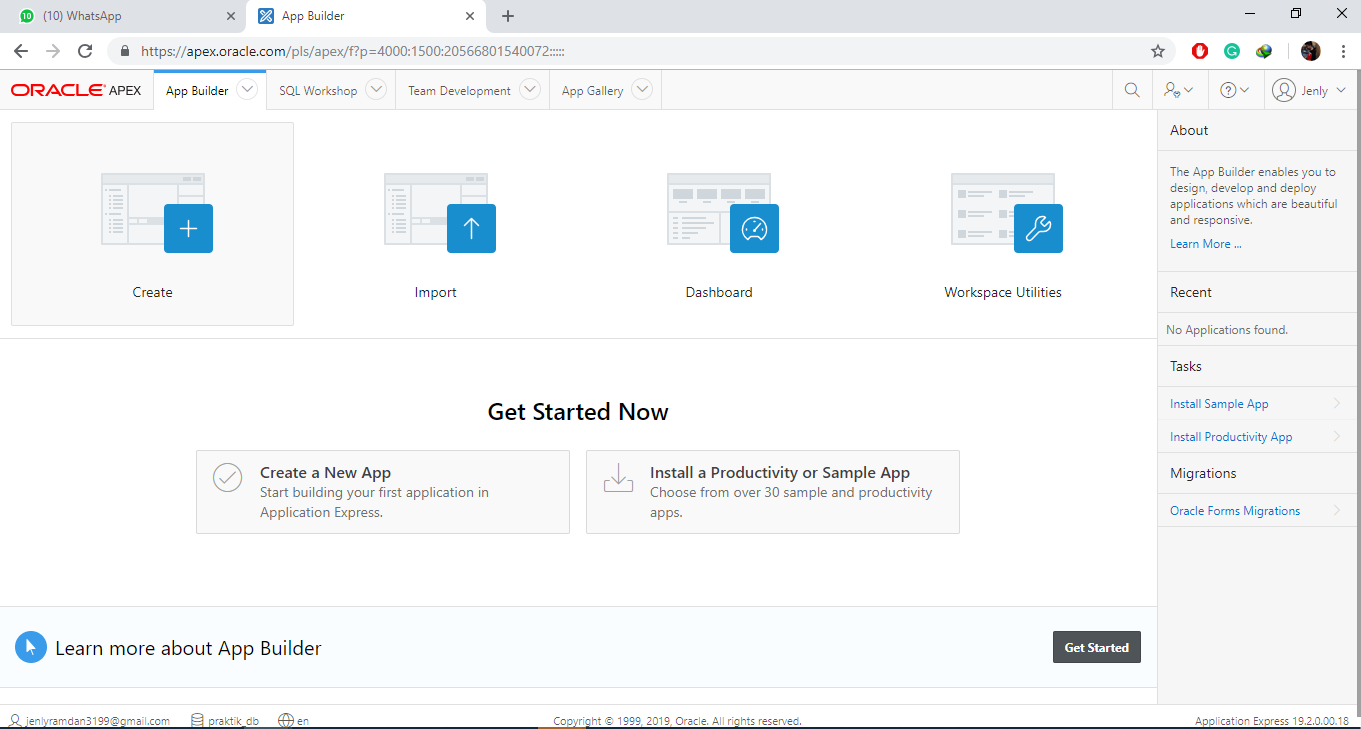
\includegraphics[width=8cm]{figures/4.png}
\end{figure}

\begin{figure}[H]
	\centering
	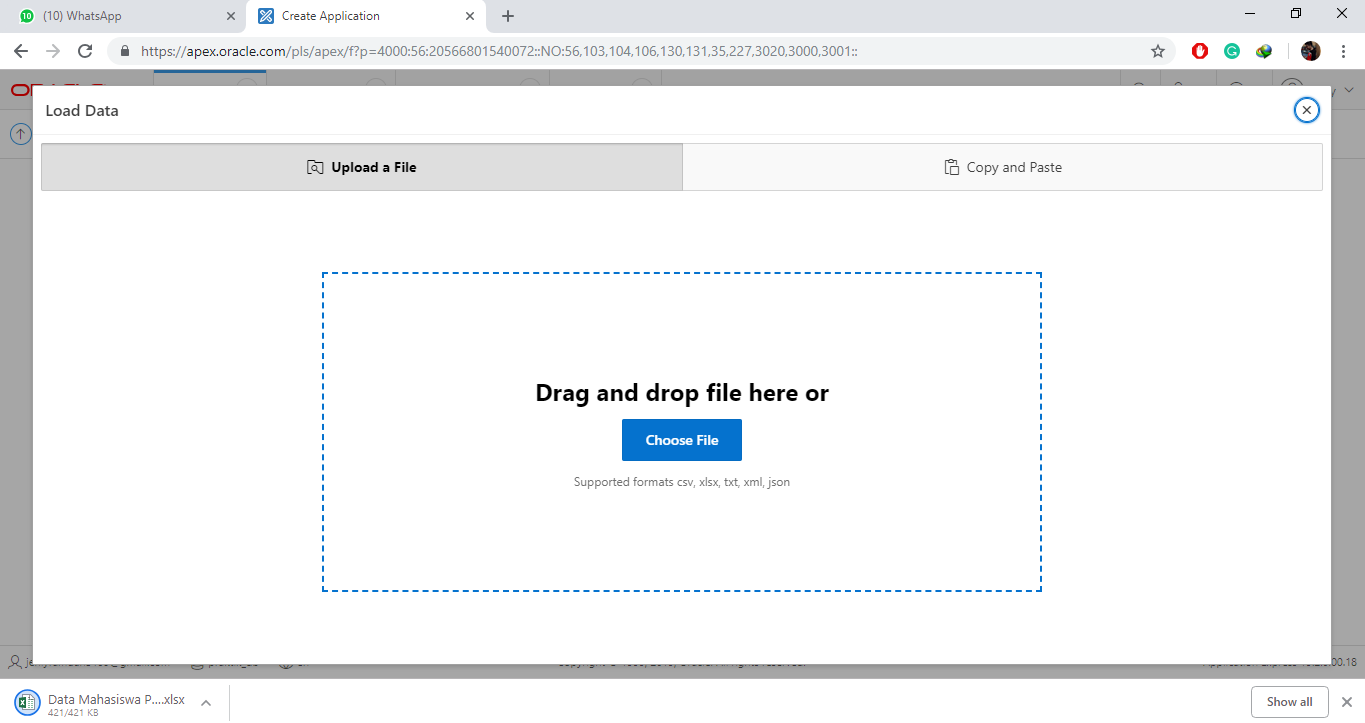
\includegraphics[width=8cm]{figures/5.png}
\end{figure}

\begin{figure}[H]
	\centering
	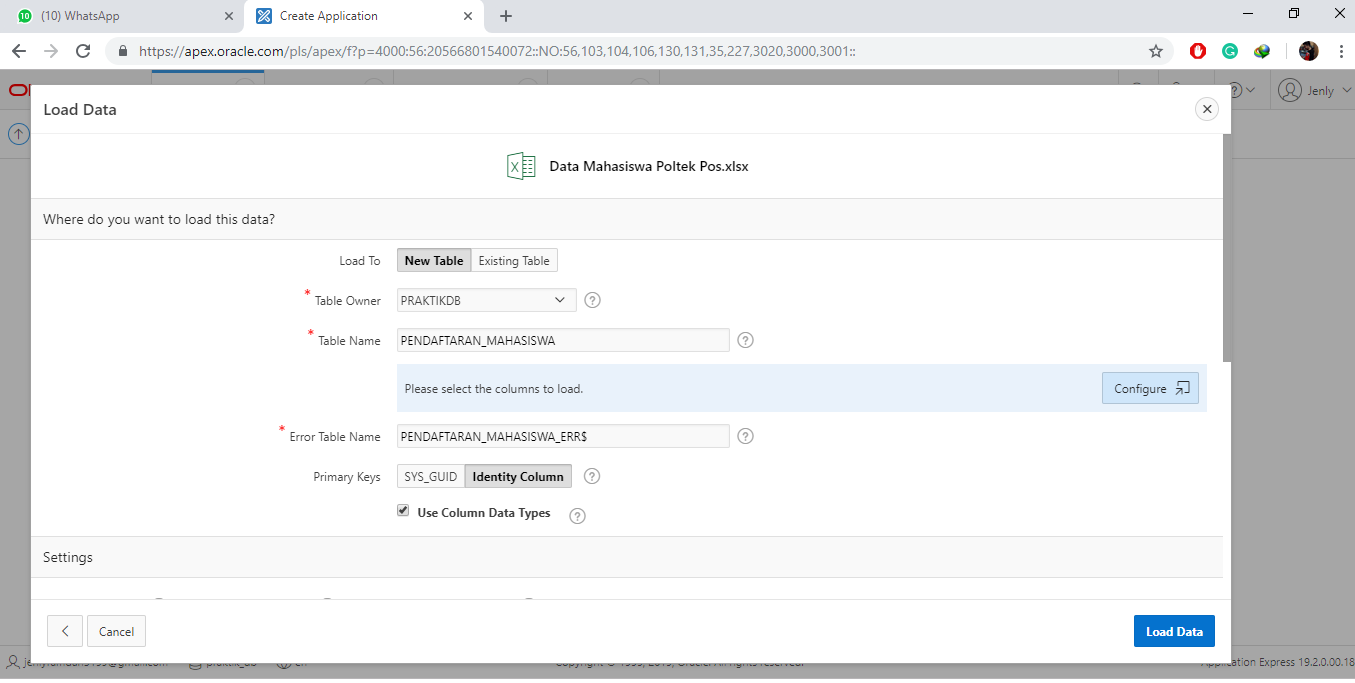
\includegraphics[width=8cm]{figures/6.png}
\end{figure}

\begin{figure}[H]
	\centering
	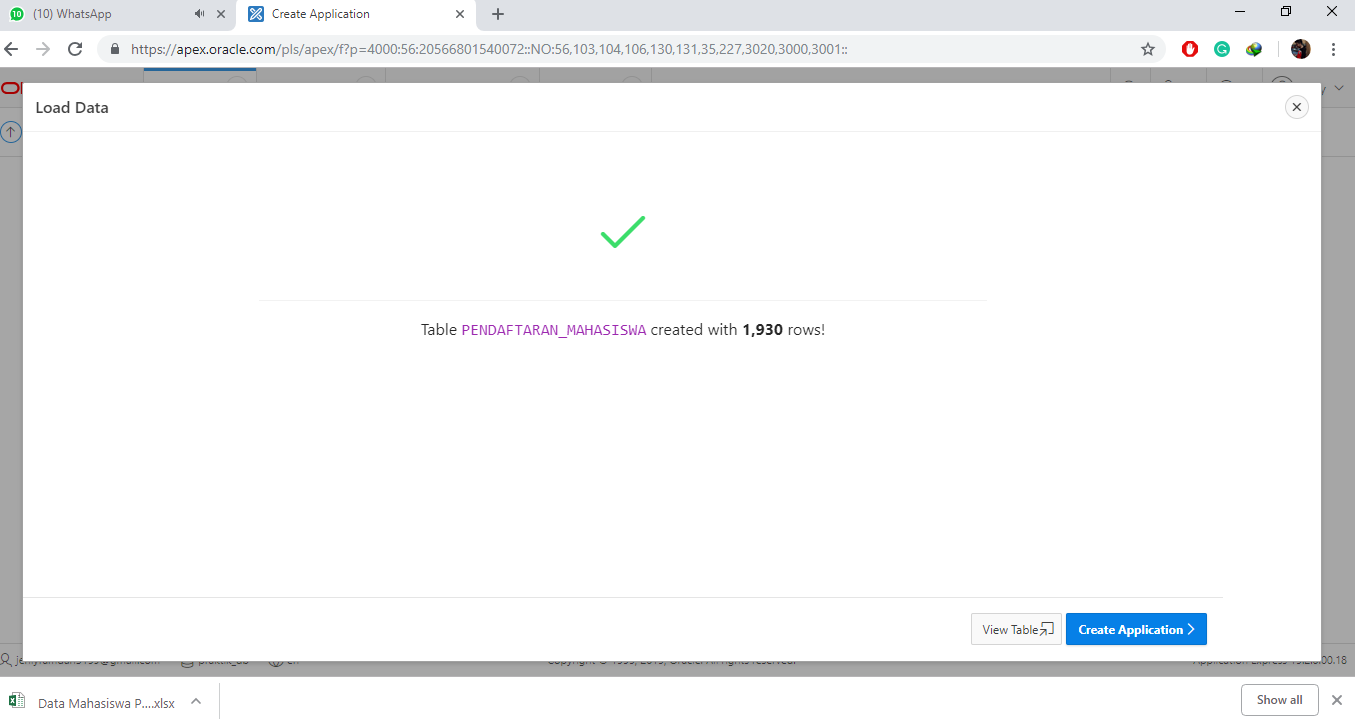
\includegraphics[width=8cm]{figures/7.png}
\end{figure}

\begin{figure}[H]
	\centering
	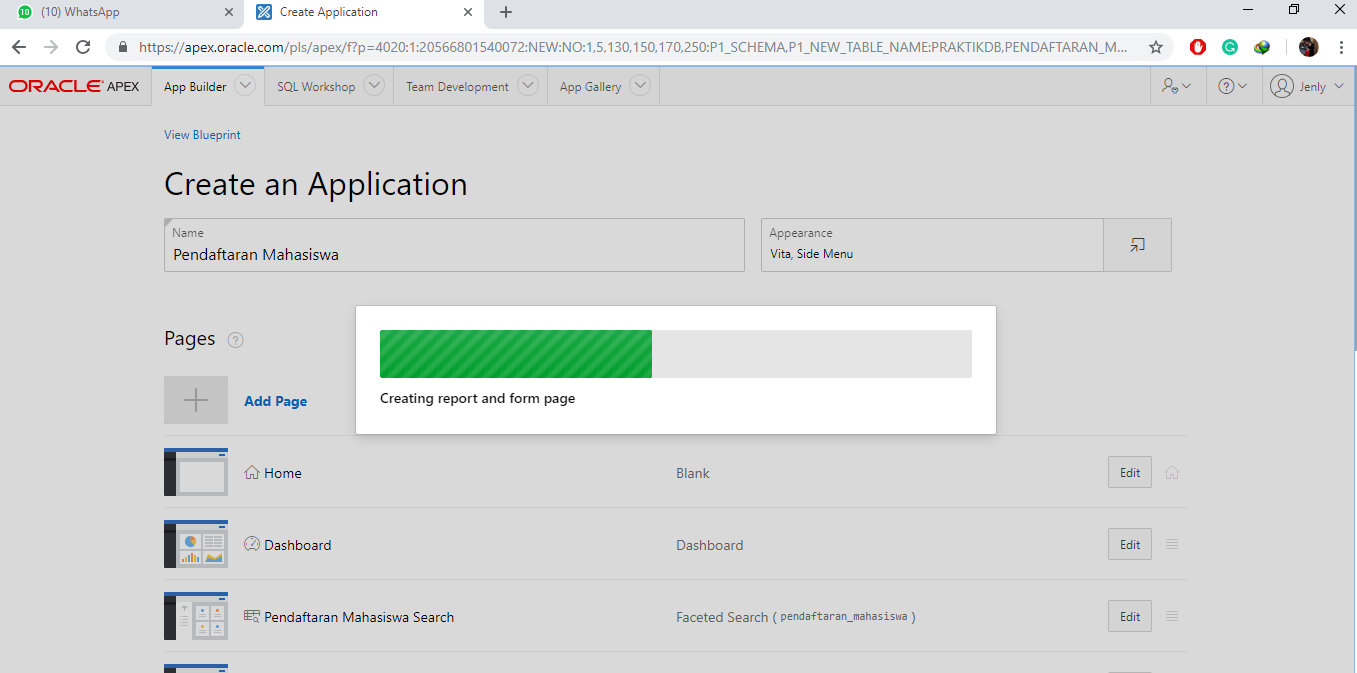
\includegraphics[width=8cm]{figures/8.png}
\end{figure}

\begin{figure}[H]
	\centering
	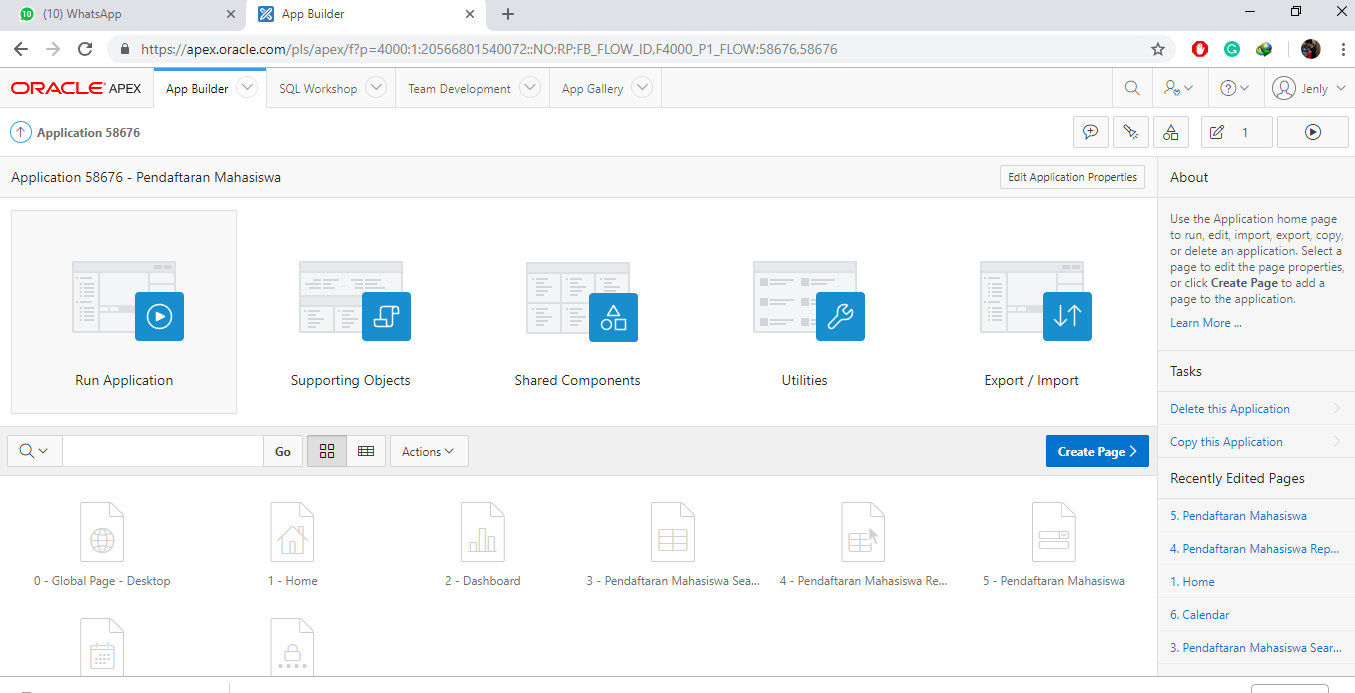
\includegraphics[width=8cm]{figures/9.png}
\end{figure}

\begin{figure}[H]
	\centering
	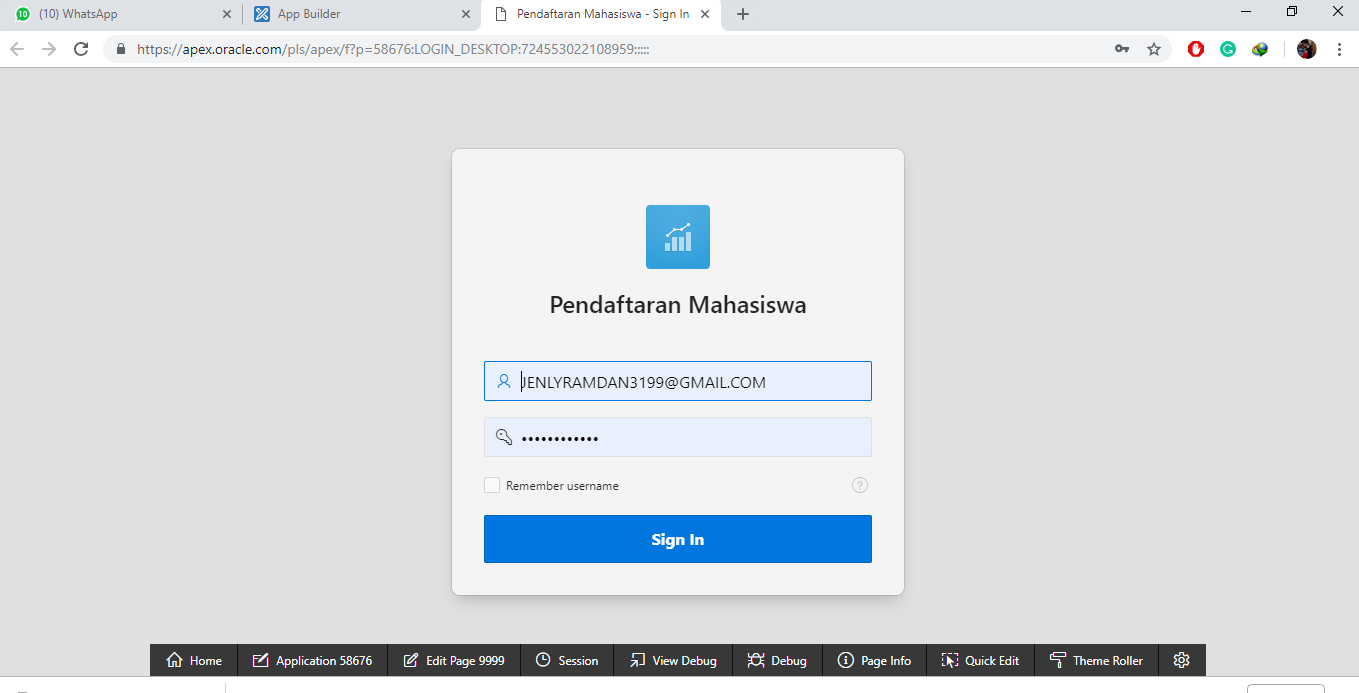
\includegraphics[width=8cm]{figures/10.png}
\end{figure}

\begin{figure}[H]
	\centering
	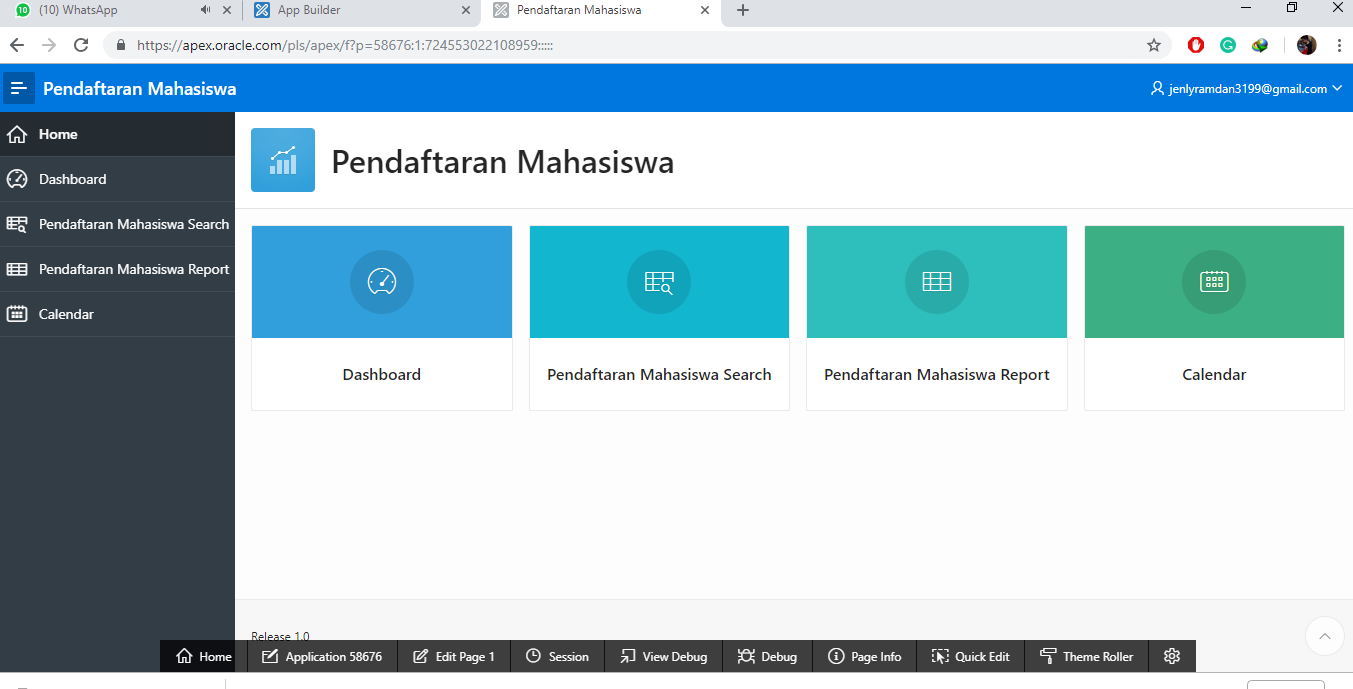
\includegraphics[width=8cm]{figures/11.png}
\end{figure}